\documentclass[a4paper, 11pt, twocolumn]{article}
\usepackage[margin=0.8in]{geometry}
\usepackage{xcolor}
\usepackage{graphicx} %package to manage images
\graphicspath{ {./images/} }

\title{A2-09 Further Mains Power Supplies}
\author{Revision sheet}
\date{}

\usepackage{fancyhdr}
\pagestyle{fancy}
\fancyhead{} % clear all header fields
\renewcommand{\headrulewidth}{0pt} % no line in header area
\fancyfoot{} % clear all footer fields
\renewcommand{\footrulewidth}{0.4pt}
\fancyfoot[C]{\thepage} % page number in centre of the page
\fancyfoot[R]{\footnotesize Thomas Boxall \\ Images from WJEC E-Book} % right hand footer has author name on top line and images reference on bottom line
\fancyfoot[L]{\footnotesize A2-09 Further Mains Power Supplies \\ Revision sheet} % left hand footer has title of document on top line and 'Revision Sheet' on bottom line

\begin{document}
    
    \maketitle

    \section{Recap from AS}
    \thispagestyle{fancy}
    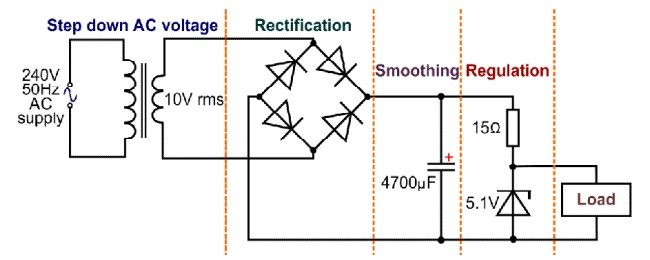
\includegraphics[width=0.4\textwidth]{recapFromAS.jpg} \\
    There are a few issues with this design, specifically the regulation subsystem:
    \begin{itemize}
        \item The Zener diode can't sustain output current \& voltage when a drop in line voltage occurs
        \item Lots of power has to be dissipated in the resistor and zener diode.
    \end{itemize}

    \section{Improvements on regulation}
    The performance of a Zener voltage regulator can be improved by incorporating an emitter follower into the output circuit. This reduces the power rating of the zener diode and resistor.
    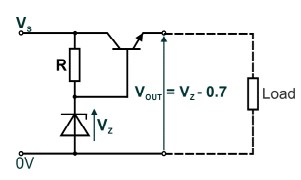
\includegraphics[width=0.4\textwidth]{emitterFollower1.jpg} \\
    $V_{out} = V_Z - 0.7$\\
    $I_C = I_L$\\
    This design can be improved further by using an Op-amp.

    \section{Op-amp stabilised power supply}
    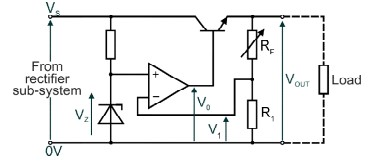
\includegraphics[width=0.4\textwidth]{opampStabilised.jpg} \\
    $\displaystyle V_1 = V_{out} \times \frac{R_1}{R_f + R_1}$ \\
    $\displaystyle V_{out} = (1+\frac{R_f}{R1})$ \\
    Advantages of using this design:
    \begin{itemize}
        \item Op-amp keeps voltage very stable
        \item Op-amp supplies base current
        \item Op-amp draws no current
    \end{itemize}

    \section{Load and Line regulation}
    \textbf{Line regulation }measures the ability of the power supply to maintain a steady output voltage when the input line voltage changes. \\
    \textbf{Load regulation }measures the ability of the output voltage to remain constant when the output current changes due to a change in the load.





\end{document}